\documentclass[a4paper]{extarticle}

\usepackage[utf8]{inputenc}
\usepackage[dutch]{babel}
\usepackage{fourier}
\usepackage{graphicx}
\usepackage[cm,empty]{fullpage}
\usepackage{xcolor}
\usepackage{multicol}
\usepackage{minted}
\usepackage{hyperref}
\usemintedstyle{vs}

\hypersetup{
	colorlinks = true
}

\definecolor{light-gray}{gray}{0.90}

\title{Git installeren}
\author{Sticky: CommIT}
\date{}

\setlength{\parindent}{0pt}
\setlength{\parskip}{0.5em}

\newcommand{\shell}[1]{\mintinline{bash}{#1}}
\newcommand{\lett}[1]{\texttt{#1}}

\begin{document}
\maketitle
\thispagestyle{empty} % https://tex.stackexchange.com/a/1737

\tableofcontents

\section{Downloaden en installeren}

\subsection{Windows}
Download het installatiepakket voor Windows via: \href{https://git-scm.com/downloads}{\lett{git-scm.com/downloads/win}}.

Download de installer die je hier krijgt, voer hem uit. Accepteer overal de standaardopties, behalve op de volgende
punten\footnote{Dit is niet per se nodig, maar zorgt ervoor dat je gemakkelijker aan de slag kunt.}:

\begin{itemize}
	\item Schakel bij de featureselectie Git GUI uit, dit wordt weinig tot niet gebruikt.

		\begin{center}
			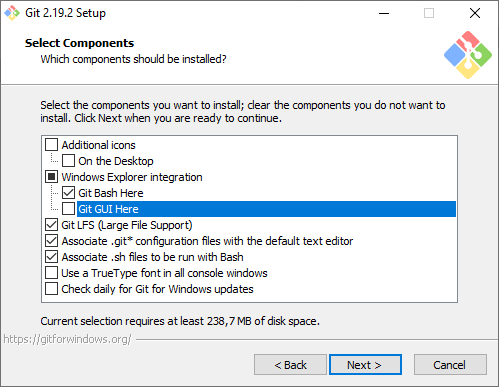
\includegraphics[width=0.75\linewidth]{windows-screenshots/1}
		\end{center}

		\newpage

	\item Selecteer een teksteditor om te gebruiken. Deze editor zal worden gebruikt om in te beschrijven wat je hebt
		veranderd, het is handig om hier een editor te kiezen die je goed kent.

		Kies hier bij voorkeur \textbf{niet} Vim, dit is een editor die zich nogal anders gedraagt dan de meeste
		editors. Kies als je geen van de genoemde editors hebt geïnstalleerd voor Nano.

		De editors die worden genoemd zijn te vinden op deze sites:
		\begin{itemize}
			\item Nano: meegeleverd
			\item Vim: meegeleverd, \url{https://vim.org/}
			\item Notepad++: \url{https://notepad-plus-plus.org/}
			\item Visual Studio Code: \url{https://code.visualstudio.com/} (let op, niet hetzelfde als Visual Studio!)
			\item Sublime Text: \url{https://sublimetext.com} (betaald)
			\item Atom: \url{https://atom.io}
		\end{itemize}
		\begin{center}
			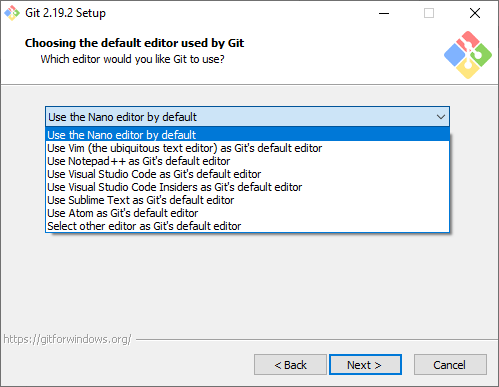
\includegraphics[width=0.75\linewidth]{windows-screenshots/2}
		\end{center}

		\clearpage

	\item Kies in dit scherm voor de eerste optie, tenzij je Git graag via \texttt{cmd} of Powershell wilt gebruiken
		(kies dan de tweede optie).

		\begin{center}
			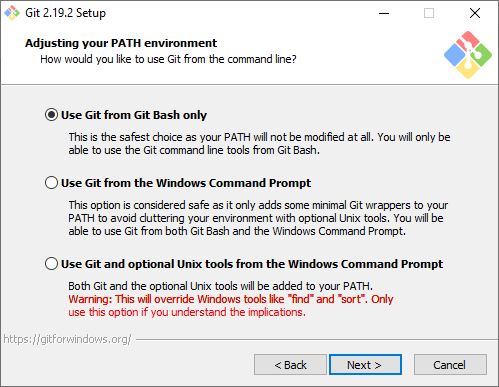
\includegraphics[width=0.75\linewidth]{windows-screenshots/3}
		\end{center}

	\item Kies voor OpenSSL als HTTPS-library.
		\begin{center}
			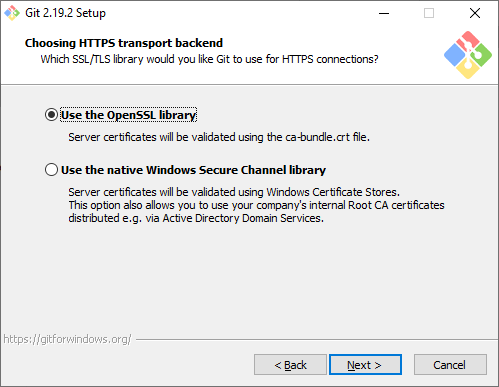
\includegraphics[width=0.75\linewidth]{windows-screenshots/4}
		\end{center}

		\clearpage

	\item Kies voor de eerste optie bij \textit{line ending conversions}, dit zorgt ervoor dat je juist samen kunt
		werken met computers die geen Windows gebruiken.

		\begin{center}
			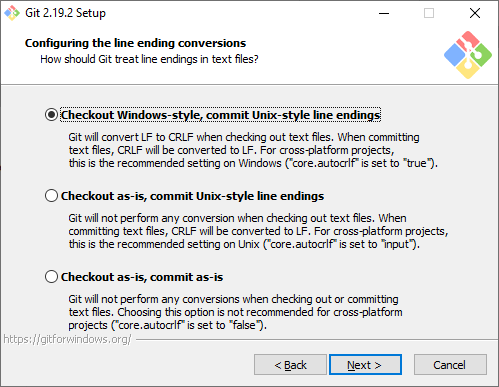
\includegraphics[width=0.75\linewidth]{windows-screenshots/5}
		\end{center}

	\item Kies voor MinTTY als terminal.
		\begin{center}
			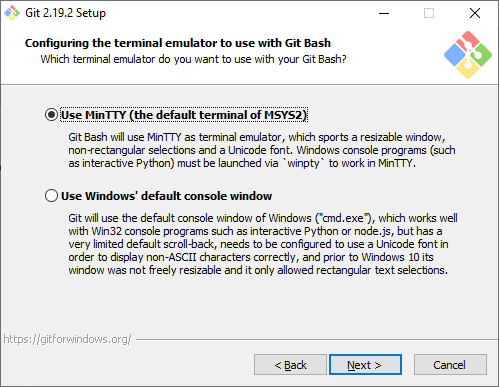
\includegraphics[width=0.75\linewidth]{windows-screenshots/6}
		\end{center}

		\clearpage

	\item Kies bij extra opties voor de eerste twee opties, en niet voor de derde optie.
		\begin{center}
			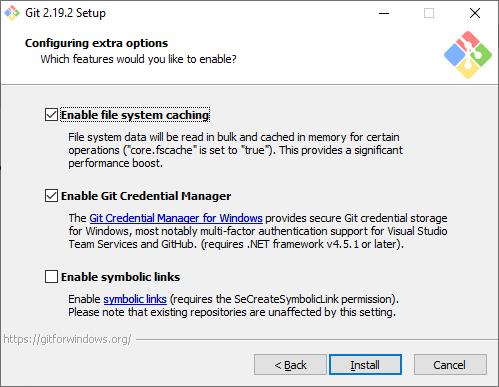
\includegraphics[width=0.75\linewidth]{windows-screenshots/7}
		\end{center}

	\item Hierna ben je klaar! Open Git Bash en ga door naar de \hyperref[instellen]{instelinstructies}.
		\begin{center}
			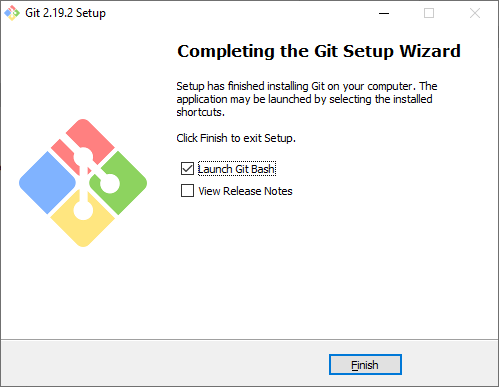
\includegraphics[width=0.75\linewidth]{windows-screenshots/8}
		\end{center}
\end{itemize}

\clearpage
\subsection{Linux}
Gefeliciteerd, je gebruikt een superieur besturingssysteem! Je hoeft geen aparte programma's behalve Git te installeren
om Git te kunnen gebruiken, gebruik de package manager van je systeem om Git te downloaden en te installeren.

Git wordt vaak ook al meegeleverd, je kan eerst proberen om \shell{git --version} uit te voeren om te zien of je Git al
hebt.

%\begin{center}
	\begin{tabular}{ll}
	 Op Debian, Ubuntu en afgeleiden: 			&\shell{sudo apt install git} \\
	 Op RHEL, CentOS, Fedora en afgeleiden: 	&\shell{sudo dnf install git} \\
	 Op Arch Linux en afgeleiden: 				&\shell{sudo pacman -S git}
	\end{tabular}
%\end{center}

Ga hierna door naar de \hyperref[instellen]{instelinstructies}.

\subsection{macOS}
Apple levert Git standaard mee, controleer of je Git hebt geïnstalleerd door Terminal te openen en het volgende commando
in te typen, en hierna op Enter te drukken:

\begin{minted}{bash}
	$ git --version
\end{minted}

Als je nog geen Git hebt zou het als het goed is geïnstalleerd moeten worden, als je Git al wel hebt zie je een bericht
dat lijkt op ``git version 2.17.1 (Apple Git)''.

Als dit niet lukt kan je Git ook installeren via
\href{https://git-scm.com/downloads/mac}{\texttt{git-scm.com/downloads/mac}}.\\
Installeer dit op de normale manier, als je vragen wordt gesteld kan je de standaardopties accepteren.

Ga hierna door naar de \hyperref[instellen]{instelinstructies}.

\section{Instellingen}
\label{instellen}
Tijdens de workshop Git zullen we Git via de CLI (\textit{command-line interface}) gebruiken. Dit is niet hoe Git in de
meeste gevallen wordt gebruikt, maar wel belangrijk om te begrijpen: de CLI-versie van Git staat aan de basis van alle
andere programma's die Git gebruiken, en de concepten erin zijn overal hetzelfde.

Open een Terminal-venster door:

\begin{itemize}
	\item Op Windows: Git Bash via het Startmenu te openen
	\item Op macOS: Terminal te openen
	\item Op Linux: je favoriete terminal te openen, vaak ook te vinden onder Ctrl-Alt-T.
\end{itemize}

Je krijgt nu als het goed is een venster te zien dat er ongeveer uitziet zoals dit:
\begin{center}
	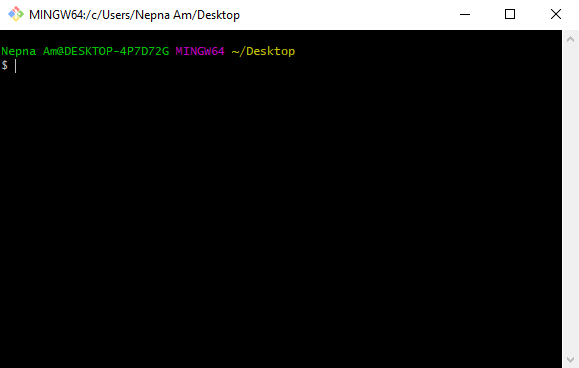
\includegraphics[width=0.75\linewidth]{terminal}
\end{center}

Hierin kan je `dingen doen' door commando's in te typen, en hierna op Enter te drukken. Hierover komt tijdens de
workshop meer uitleg.

Als voorbeeld kan je het commando \texttt{ls} uitvoeren, dit laat de bestanden in de map waar je zit zien. Dit doe je
door \texttt{ls} te typen, en hierna op Enter te drukken. Als het goed is krijg je dan een paar regels tekst te zien,
met hierin de namen van bestanden die in de standaardmap van je gebruiker zijn opgeslagen, en hierna weer een nieuwe
regel om tekst op in te voeren.

Voer de volgende commando's in om Git in te stellen:

\begin{itemize}
	\item \shell{git config --global user.name "Jouw Naam"}\\
		Vervang `\texttt{Jouw Naam}' met je naam, maar laat de aanhalingstekens staan!

		Dit commando stelt de naam in die Git verbindt aan jouw code. Deze naam is zichtbaar voor iedereen met wie je
		samenwerkt, dus het is handig om hier je volledige naam in in te stellen.

	\item \shell{git config --global user.email "emailadres@example.com"}

		Vul ook hier weer je eigen e-mailadres in. Je e-mailadres en naam zijn beiden zichtbaar voor iedereen met wie je
		samenwerkt, dit omdat Git oorspronkelijk is bedoeld voor grote projecten. Het is niet verplicht om hier je echte
		e-mailadres in te vullen, maar wel aan te raden, sommige websites waar je je code op kan zetten werken niet
		altijd juist als dit e-mailadres niet klopt.

	\item \shell{git config --global credential.helper "cache --timeout=3600"}

		Dit commando zorgt ervoor dat Git je gebruikersnaam en wachtwoord een uur (3600 seconden) lang onthoudt wanneer
		je contact hebt met een externe server. Je kan het aantal seconden ook ophogen om nog minder vaak om je
		wachtwoord te worden gevraagd.

		Het is ook mogelijk om Git zo in te stellen dat je überhaupt geen wachtwoord nodig hebt om je code te kunnen
		versturen / ophalen, dit is iets ingewikkelder en behandelen we niet tijdens de workshop. Zie hiervoor de
		instructies van Github over SSH-keys op \url{https://help.github.com/articles/about-ssh/}.

	\item \shell{git config --global color.ui auto}

		Dit commando schakelt kleuren in de uitvoer van Git in. Wanneer je bijvoorbeeld iets toevoegt wordt dit groen
		gemaakt, en verwijderde code wordt rood.

	\item \shell{git config --global commit.verbose true}

		Dit commando zorgt ervoor dat wanneer je een punt vast wilt leggen in de geschiedenis, je alle wijzigingen te
		zien krijgt die je hebt klaargezet om op te slaan. Hierover komt meer uitleg tijdens de workshop.
\end{itemize}

Voer als je niet op Windows zit en Git nog niet eerder hebt gebruikt ook het volgende commando uit:
\begin{itemize}
	\item \shell{git config --global core.editor "nano"}

		Dit commando stelt de teksteditor in die je zal gebruiken om te beschrijven wat je hebt gedaan. \shell{nano} is
		een simpele editor in de terminal die gemakkelijk is te gebruiken, andere opties zijn:

		\begin{itemize}
			\item \shell{git config --global core.editor "code --wait"} voor \href{https://code.visualstudio.com}{Visual Studio Code},
			\item \shell{git config --global core.editor "atom --wait"} voor \href{https://atom.io}{Atom},
			\item \shell{git config --global core.editor "gedit -s"} voor Gedit.
		\end{itemize}
\end{itemize}
\end{document}
